\begin{example}
 Βρείτε το συμμετρικό του πολυγώνου $V$ με κορυφές $A(-1, 0)$, $B(0, -2)$, $C(1, 0)$ και $D(0, 2)$ ως προς:
\begin{enumerate}
    \item[α)] οριζόντια ευθεία $y=2$
    \item[β)] κατακόρυφη ευθεία $x=2$
    \item[γ)] ευθεία $y=x+2$
\end{enumerate}
\end{example}


\begin{solution}
Το πολύγωνο παρουσιάζεται υπό μορφή πίνακα ως εξής:

\[
V = \begin{bmatrix}
-1 & 0 & 1 & 0 \\
0 & -2 & 0 & 2 \\
1 & 1 & 1 & 1
\end{bmatrix}
\]

Θα χρησιμοποιήσουμε τον πίνακα $M_L$ όπως έχει ορισθεί στο Παράδειγμα 5.
\begin{enumerate}
    \item[α)] Η ευθεία $y=2$ έχει σημείο τομής με τον άξονα των $y$ το $(0,2)$ και σχηματίζει γωνία $\theta = 0$ με τον $x$. Επομένως $\theta=0$, $m=0$ και $v=2\hat{j}$. Αντικαθιστώντας αυτές τις τιμές στον πίνακα $M_l$ προκύπτει:
    \[
    M_L = \begin{bmatrix}
    1 & 0 & 0 \\
    0 & -1 & 4 \\
    0 & 0 & 1
    \end{bmatrix}
    \]
Αυτός ο πίνακας αναστρέφει το πολύγωνο συμμετρικά ως προς $y=2$.
Οι συντεταγμένες του καινούργιου πολυγώνου προκύπτουν από τη σχέση:

\[
V' = A'B'C'D' = M_L \cdot V = \begin{bmatrix}
1 & 0 & 0 \\
0 & -1 & 4 \\
0 & 0 & 1
\end{bmatrix}
\begin{bmatrix}
-1 & 0 & 1 & 0 \\
0 & -2 & 0 & 2 \\
1 & 1 & 1 & 1
\end{bmatrix}
= \begin{bmatrix}
-1 & 0 & 1 & 0 \\
4 & 6 & 4 & 2 \\
1 & 1 & 1 & 1
\end{bmatrix}
\]

Τελικό $A' = (-1, 4)$, $B' = (0, 6)$, $C' = (1, 4)$ και $D' = (0, 2)$.

    \item[β)] Η ευθεία $x=2$ (Σχήμα ) είναι παράλληλη με τον άξονα των $y$ άρα δεν έχει σημείο τομής. Επίσης, έχει άπειρη κλίση! Γι' αυτό αν $v = 2\hat{i}$ θα πρέπει να εκτελεστεί ο ακόλουθος μετασχηματισμός:\\
Βήμα 1: Μεταφορά κατά διάνυσμα $-v$, ώστε η ευθεία $x=2$ να πάει πάνω στον άξονα $y$. 
\[
\text{Βασικός πίνακας μετασχηματισμού: } T_{-v}
\]
Βήμα 2: Συμμετρία ως προς $y$.
\[
\text{Βασικός πίνακας μετασχηματισμού: } M_y
\]
Βήμα 3: Επαναφορά της ευθείας $x=2$ στην αρχική της θέση, δηλαδή μεταφορά κατά διάνυσμα $v$.
\[
\text{Βασικός πίνακας μετασχηματισμού: } T_v
\]

Ο ζητούμενος μετασχηματισμός $M$ προκύπτει σαν σύνθεση των παραπάνω, δηλαδή:

\[
M = T_v \cdot M_y \cdot T_{-v} = \begin{bmatrix}
1 & 0 & 2 \\
0 & 1 & 0 \\
0 & 0 & 1
\end{bmatrix}
\begin{bmatrix}
1 & 0 & 0 \\
0 & -1 & 0 \\
0 & 0 & 1
\end{bmatrix}
\begin{bmatrix}
1 & 0 & -2 \\
0 & 1 & 0 \\
0 & 0 & 1
\end{bmatrix} = \begin{bmatrix}
1 & 0 & 0 \\
0 & -1 & 0 \\
0 & 0 & 1
\end{bmatrix}
\]

Οι συντεταγμένες του καινούργιου πολυγώνου δίνονται από:
\[
V' = A'B'C'D' = MV = \begin{bmatrix}
1 & 0 & 0 \\
0 & -1 & 0 \\
0 & 0 & 1
\end{bmatrix}
\begin{bmatrix}
-1 & 0 & 1 & 0 \\
0 & 2 & 0 & 2 \\
1 & 1 & 1 & 1
\end{bmatrix} = \begin{bmatrix}
-1 & 0 & 1 & 0 \\
0 & -2 & 0 & -2 \\
1 & 1 & 1 & 1
\end{bmatrix}
\]

Τελικό $A' = (-1, 0)$, $B' = (0, -2)$, $C' = (1, 0)$ και $D' = (0, -2)$.

    \item[γ)] Η ευθεία $y=x+2$ έχει κλίση $m=1$ και σημείο τομής με τον άξονα των $y$ το $(0,2)$, επομένως $b=2$. Ο πίνακας $M_l$ του παραδείγματος 5 παίρνει την ακόλουθη τιμή:
\[
M_l = \begin{bmatrix}
0 & 1 & -2 \\
1 & 0 & 2 \\
0 & 0 & 1
\end{bmatrix}
\]

Οι συντεταγμένες του καινούργιου πολυγώνου δίνονται από:
\[
V' = A'B'C'D' = M_l V = \begin{bmatrix}
0 & 1 & -2 \\
1 & 0 & 2 \\
0 & 0 & 1
\end{bmatrix}
\begin{bmatrix}
-1 & 0 & 1 & 0 \\
0 & 2 & 0 & 2 \\
1 & 1 & 1 & 1
\end{bmatrix} = \begin{bmatrix}
2 & 2 & 0 & 2 \\
-1 & 0 & -2 & 0 \\
1 & 1 & 1 & 1
\end{bmatrix}
\]

Τελικό $A' = (2, -1)$, $B' = (2, 0)$, $C' = (0, -2)$ και $D' = (2, 0)$.

Μια στρέβλωση (shearing) κατά μήκος του $X$-άξονα, του σημείου $\overline{P}(x, y)$ με παράγοντα στρέβλωσης $a$, φέρνει το σημείο $\overline{P}$ στο $\overline{P'}(x', y')$ και ισχύει:
\[
x' = x + ay, \quad y' = y .
\]

Χρησιμοποιώντας πίνακες γράφουμε:
\[
\begin{bmatrix}
x' \\
y'
\end{bmatrix} = \begin{bmatrix}
1 & a \\
0 & 1
\end{bmatrix}
\begin{bmatrix}
x \\
y
\end{bmatrix}
\]

ή \(\overline{P'} = SH_x \cdot \overline{P}\) με:
\[
SH_x = \begin{bmatrix}
1 & a \\
0 & 1
\end{bmatrix}
\]

Για την περίπτωση της στρέβλωσης κατά μήκος του $Y$-άξονα και με παράγοντα στρέβλωσης $b$ ισχύει:
\[
SH_y = \begin{bmatrix}
1 & 0 \\
b & 1
\end{bmatrix}
\]


Στο σχήμα  δείχνεται η στρέβλωση ενός τετραγώνου για τις δύο περιπτώσεις $a=2$ και $b=2$.

\begin{figure}[h!]
	\begin{center}
		\begin{minipage}[b]{0.19\textwidth} % Top-left image
		    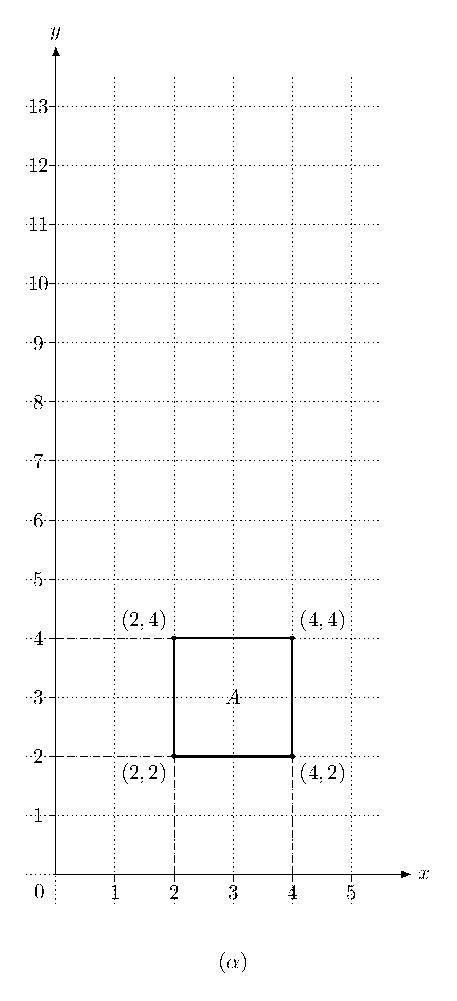
\includegraphics[width=\textwidth]{Chapter2/figure17a.pdf}
		\end{minipage}%
	\hfill
		\begin{minipage}[b]{0.4\textwidth} % Top-right image
		    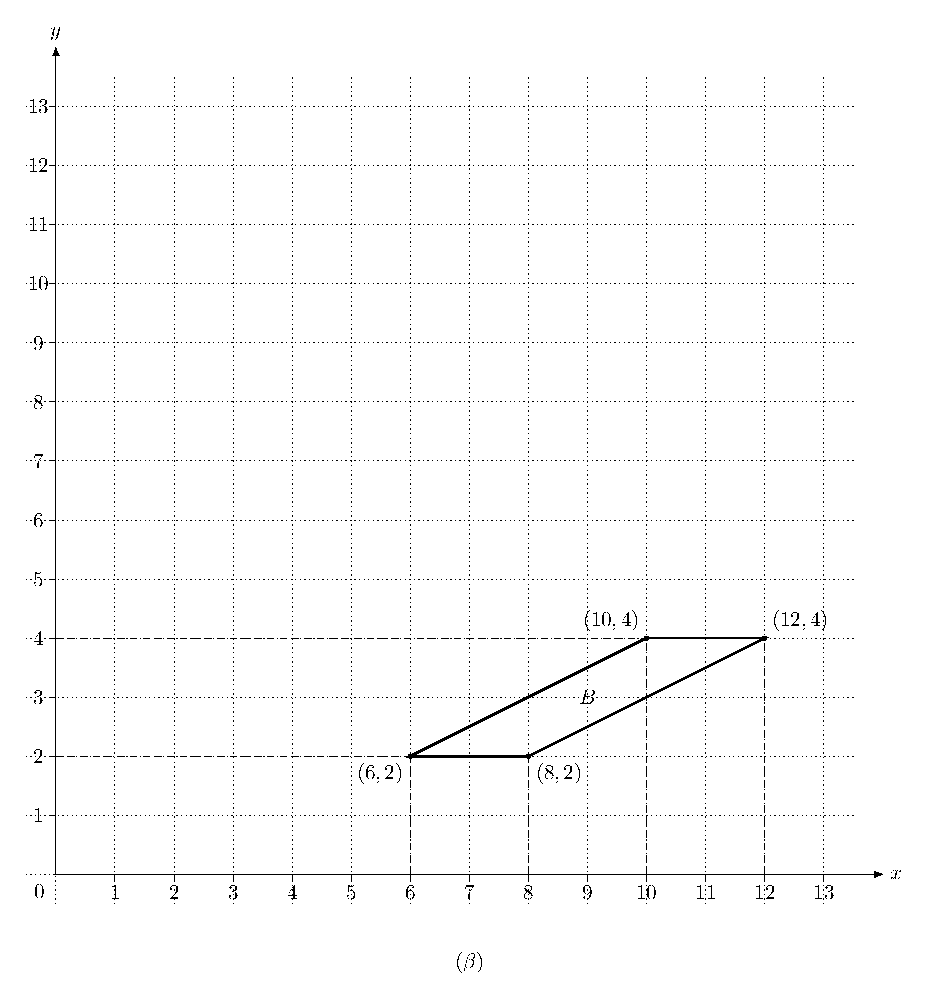
\includegraphics[width=\textwidth]{Chapter2/figure17b.pdf}
		\end{minipage}
	\hfill
		\begin{minipage}[b]{0.4\textwidth} % Top-right image
		    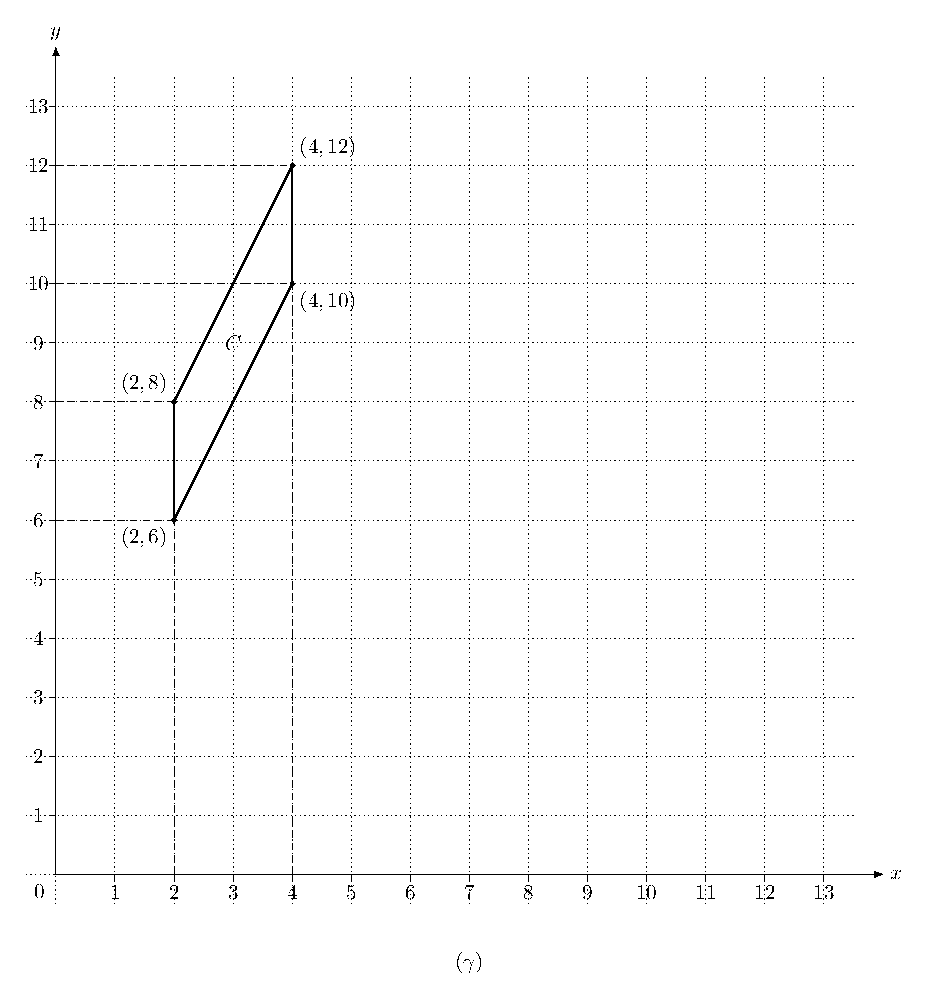
\includegraphics[width=\textwidth]{Chapter2/figure17c.pdf}
		\end{minipage}
	\end{center}
\caption{Στρέβλωση ενός τετραγώνου για $a=2$ και $b=2$}
\end{figure}

\end{enumerate}

\end{solution}
